\documentclass[a4paper,12pt]{article}
\usepackage{amssymb}
\usepackage{tikz}
\usepackage{forest}
\usetikzlibrary{arrows.meta,shapes.arrows,chains,decorations.pathreplacing,matrix}
  \newlength\myht{}
\settoheight{\myht}{\(n-2\)} 
\tikzset{%
  MyStyle/.style={draw, text width=15pt, text height=10pt, text centered,minimum height=\myht+2*2*1mm},
  myarrow/.style={shape=single arrow, rotate=90, inner sep=5pt, outer sep=0pt, single arrow head extend=0pt, minimum height=0pt, text width=0pt, draw=blue!50, fill=blue!25}
}

\forestset{%
  default preamble={
    for tree={
      circle,
      draw,
      inner sep=0pt,
      minimum size=.5cm,
      font=\scriptsize,
      edge=->,
      anchor=north
    }
  },
  triangle/.style={isosceles triangle,
                  draw,
                  shape border rotate=90,
                  minimum size=.7cm,
                  child anchor=apex,
                  anchor=apex}
}

\title{Homework Two} 
\author{Robert George Phillips (rogphill@ucsc.edu)}
\date{February 21, 2018}

\begin{document}
\maketitle

\textbf{Question 1 (2 points):} Heaps naturally lead to a sorting algorithm, Heapsort. Starting from array A, build it into a min-heap. Repeatly called Extract-Min to get the elements of A in sorted order. Give pseudocode for Heapsort and show that it is not stable.\\

\textbf{Analysis:} We start with an array $A = \{A_0, A_1, \ldots, A_k\}$ with $k$ elements. We can turn this into a heap by iterating through each element and forming a tree structure where each node has two children. We can see this more easily with a sample array: \\

$$ 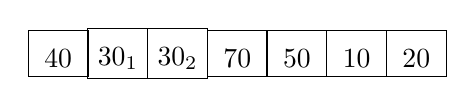
\begin{tikzpicture}[-{Stealth[length=2.5pt]}]
      \begin{scope} [start chain, node distance=-.5pt]
        \foreach \name [count=\xi] in {40, 30_1, 30_2, 70, 50, 10, 20}{ \node[MyStyle, on chain] (vlos\xi) {$\name$};}
      \end{scope}
\end{tikzpicture} $$ \\

This sample array can simply be visualized into a heap, such that:\\

$$\begin{forest}
    [{\(40\)},rectangle,draw
    [\(30_1\),rectangle,draw
        [\(70\),rectangle,draw]
        [\(50\),rectangle,draw]
        ]
    [\(30_2\),rectangle,draw
      [\(10\),rectangle,draw]
      [\(20\),rectangle,draw]
    ]
    ]
\end{forest}  $$\\

We have visualized a heap structure, but need to turn it into a min-heap, where the minimum element of the heap, $10$, is at the root node. We can use min-heapify for this.

Min-heapify assumes that the subtree rooted at $i$ has children that are heaps, but may not be a heap itself, and uses the fact that our base case is a single node that has no children -- which is why we start at $n -1$ and decrement to $0$. Additionally, if the element $A[i].key$ is at least the minimum of the children's keys, we are done. Otherwise, min-heapify will find a child $j$ of $A[i]$ with a minimum key and swap $A[i]$ with $A[j]$. Finally, it will call itself recurisively. In this way, the minimum value floats up and the larger values float down. In pseudocode: \\

\begin{verbatim}
Min-Heapify(A, i): //running time: O(logn)
     if A[i] has no children, return
     
     if A[i].key <= A[i].leftchild.key && A[i].rightchild.key, return
     
     else, find child j of A[i] with min key and swap(A[i], A[j])
     Min-Heapify(A, j)
\end{verbatim} 

This type of data structure naturally leads to a sorting algorithm. We can run a heapsort with the following pseudocode:\\

\begin{verbatim}
for i = n - 1 to 0:
     min-heapify(A, i) //this procedure takes O(nlogn)
\end{verbatim} 

Our first legitimate run through heapsort brings us to this min-heap subtree, where $30_2$ was swapped with it's smaller child node $10$:\\

$$\begin{forest}
    [{\(10\)},rectangle,draw
    [\(30_2\),rectangle,draw
        ]
    [\(20\),rectangle,draw
    ]
    ]
  \end{forest}$$\\
  
After min-heapify iterates fully through the for loop, $10$ ''floats up'' to the root and we obtain the following heap:\\

$$\begin{forest}
    [{\(10\)},rectangle,draw
    [\(30_1\),rectangle,draw
        [\(70\),rectangle,draw]
        [\(50\),rectangle,draw]
        ]
    [\(20\),rectangle,draw
      [\(30_2\),rectangle,draw]
      [\(40\),rectangle,draw]
    ]
    ]
  \end{forest}$$\\

At every $i$, all subtrees rooted at $j$ for $j>i$ are valid and correct heaps. In a min-heap, a parent node is always less than or equal to it's children nodes, and the root of the heap is always the minimum element. A parent is accessed by $\frac{i}{2}$ and it's children are given by $2i+1$ and $2i+2$. \\

From here, we can use extractMin(), a function of a priority queue, which swaps the root node with the last node, and then returns the original root, and finally running heapify on the new root node. When this procedure is finished, we can call extractMin() again to fill up an array in sorted ascending order. The array that returns is such that:\\

$$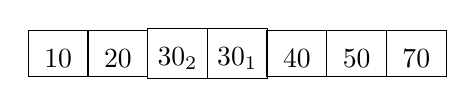
\begin{tikzpicture}[-{Stealth[length=2.5pt]}]
      \begin{scope} [start chain, node distance=-.5pt]
        \foreach \name [count=\xi] in {10, 20, 30_2, 30_1, 40, 50, 70}{ \node[MyStyle, on chain] (vlos\xi) {$\name$};}
      \end{scope}
\end{tikzpicture}$$ \\

With this example, we can also see that $30_1$ and $30_2$ are out of order and thus Heapsort is not a stable sorting algorithm.

$$\blacksquare$$

\textbf{Question 2 (2 points):} Given an input array $A$ of length $n$ and a positive integer $k > 0$, design an algorithm that outputs the largest $k$ elements in sorted order. Provide pseudocode and give a time-complexity analysis. You will get full credit if the time-complexity is $O(n+k log k)$. (If you get anything less efficient, you only get 1 point.)\\

\textbf{Analysis:} Starting with the trivial solution, we could make a simple modification to Max-Heapsort, iterating our loop from $n-1$ to $n-1-k$ instead of from $n-1$ to $0$. Inside the loop, it would swap the root node, the maximum element, with the last node in the tree, then reducing the heap size by one and run Max-Heapify on the new root node. We could then return the output in the form of $A=\{A_{n-1}, \ldots, A_{n-1-k}\}$ when the loop is finished. This algorithm would run in $O(klogn)$. Here is some pseudocode:\\

\begin{verbatim}
for i = n - 1 to n - 1 - k:
     Heapsort(A) //this procedure takes O(n+klogn)
return A[n-1 ... n-1-k]
\end{verbatim}

To achieve $O(n+klogk)$ time-complexity, I believe I would need to use two arrays $A$ and $B$, and run max-heapify on both of them until they are max heaps. Then, let heap $B$ act as a . This should run in $O(n+klogk)$.   \\

$$\blacksquare$$\\

\textbf{Question 3 (1 point):} Prove that the number of keys stored in a 2-3 tree of height $h$ is $\Omega(2^h)$ and $O(3^h)$. \\

\textbf{Invariant:} The \textit{invariant} of a 2-3 tree is that all of the children of every node have the same height $h$, and all leaf nodes lie on the same height $h$. Nodes also only ever have 0, 2, or 3 children -- barring the nodes at level $h$ which are all leaf nodes. Nodes also store one or two keys (also known as elements).\\

\textbf{Base case:} We can start with our base case, which is when $h=1$. This is trivially true as level $h=0$ of the 2-3 tree is the root node, and at level $h=1$ there can be only two children nodes in the best-case scenario, and three children nodes in the worst-case scenario, so thus our base case $\in \Omega(2^h)=\Omega(2^1)$ and $\in O(3^h)=O(3^1)$.\\ 

\textbf{Induction:} Our invariant holds true for $h = 1, \ldots, k$. The keys, or elements, of a 2-3 tree are stored in each node, so our algorithm $h \in \Omega(2^k)$ in our best-case scenario and $\in O(3^k)$ in our worst-case scenario 2-3 tree. Now we can use induction to prove that it is true for $h = 1,\ldots, k, k+1$.\\

Nodes can only ever have two or three children, and nodes store the either one or two keys. This implys $2^h$ nodes in the best-case with a runtime $\in \Omega(2^h)$, and $3^h$ nodes in the worst-case with a runtime $\in O(3^h)$. If this is the case, then when $h+1=k+1$, we have $2^{h+1}$ nodes in the best-case with a runtime $\in \Omega(2^{h+1})$ and $3^{h+1}$ nodes in the worst-case with a runtime $\in O(3^{h+1})$.\\

Thus, the number of keys stored in a 2-3 tree with a height of $h$ is $\Omega(2^h)$ and $O(3^h)$. 

$$\blacksquare$$\\

\textbf{Question 4 (2 points):} Suppose you are given two 2-3 trees $T_1$, $T_2$, and a value $x$ such that all keys in $T_1$ are less than $x$, and all keys in $T_2$ are greater than $x$. Give an algorithm that constructs a single new $T_0$ that has the union of keys in $T_1$, $T_2$, and $x$. Give a running time analysis.\\

\textbf{Analysis:} First, we can insert() $x$ into one of the smaller tree's leaves, which I will use as $T_1$ in my example. First, we will need to search through the tree to find an appropriate leaf to insert $x$ into. If a leaf already has one existing key, we simply just insert our new key $x$ into the leaf. If the leaf has two existing keys, we still insert . Finally, we run fix-overfull() on the node. This will take $O(logn)$ time. Here is what the result will look like:\\

$$\begin{forest}
    [{\(T_1\)},triangle,draw
    [\(T_1a\),triangle,draw
        ]
    [\(T_1b\),triangle,draw
    ]
    [\(x\),rectangle,draw
    ]
    ]
  \end{forest}$$ \\
  
 Now that we have $T_1 \cup x$ in a single 2-3 tree, we need to find a way to ''merge'' the unioned 2-3 tree with $T_2$. This union of $T_1$ and $x$ can also be treated as a single node, like this example:\\
 
 $$\begin{forest}
    [{\(T_1 \cup x\)},triangle,draw]
  \end{forest} $$\\
  
  Since a 2-3 tree is also technically a node, we can use this fact to insert() $T_1 \cup x$ into one of $T_2$'s leaves and call fix-overfull() after, as fix-overfull() accepts nodes as a parameter. This will take $O(logn)$ worst-case runtime. Here is a visualization of that merge if the keys in $T_1 \cup x$ are less than the keys in $T_2$ (it would go to the far right leaf if the keys in $T_1 \cup x$ are greater than the keys in $T_2$):\\
  
 $$\begin{forest}
    [{\(T_2\)},triangle,draw
    [\(T_{2a}\),triangle,draw
        [\(T_1 \cup x\),triangle,draw]
        [\(T_{2d}\),triangle,draw]
        ]
    [\(T_{2b}\),triangle,draw
      [\(T_{2e}\),triangle,draw]
      [\(T_{2f}\),triangle,draw]
    ]
    [\(T_{2c}\),triangle,draw
      [\(T_{2g}\),triangle,draw]
      [\(T_{2h}\),triangle,draw]
    ]
    ]
  \end{forest}  $$ \\
  
The 2-3 tree would be unbalanced with this addition, so we call fix-overfull() on the root node of $T_1 \cup x$, which would balance the 2-3 tree to satisfy the properties all three properties of a 2-3 tree.\\

$$\blacksquare$$ 

\textbf{Question 5 (3 points):} Consider a binary search tree where keys are positive integers. Augment the tree to answer Range queries of the form: “how many elements have key in the range [$a$, $b$]”? Thus, such a query is called by the function Range($a$, $b$).\\

Provide pseudocode for Insert, Delete, and Range queries. Provide a running time analysis for all these queries, in terms on $n$ (the number of nodes in the tree) and $D$ (the maximum depth). (Hint: you might want to maintain subtree sizes at the nodes.)\\

\textbf{Analysis:} To solve this, I would have to envision a binary search tree that, for each node, would hold the number of nodes in in a parent's subtree. Now we can start to perform our range query. It would recursively call itself, and if the node has a null key, return. If the node has a key that is less than or equal to $a$, everything to the left of it must be out of the range, so we add it to a counting variable. If the node has a key that is greater than or equal to $b$, everything to the right must be out of the range, so we add it to a counting variable. At the end of the recursion, we return the main root of the entire tree's left and right subtree size to get a total tree size, and then subtract it from our counting variable. Here is some pseudocode (the runtime would be O(D+n), and D $\leq$ n so O(n)):\\

\begin{verbatim}
count = 0;

Range(node, a,b): //this runs in O(n)
    if (node.key == null) {return}
    if (node.key<= a){ count += node.leftsize, return }
    Range(node.left,a,b)
    if (node.key>= b){ count += node.rightsize, return }
    Range(node.right,a,b)
    return mainroot.leftsize+mainroot.rightsize-count
\end{verbatim}

We would need to update tree sizes as we traverse the tree in this environment. Here is some pseudocode to display how we would modify insert to handle keeping track of a subtree's size: \\

\begin{verbatim}
insert(node, val):
    if (node.key == null) { node.key = val }
    else if (val < node.key) {
        node.leftsize++
        insert(node.left, val)    
    } else {
        node.rightsize++
        insert(node.right, val)
    }
\end{verbatim}

Additionally, we would need a delete function that checks if there are no children, one child, or two children in the tree before deletion. This runtime of this would be $O(n)$. Here is some pseudocode to display how we would modify delete to handle keeping track of a subtree's size: \\

\begin{verbatim}
delete(node, val): //this is an O(n) operation
    if (node.key == val) { 
        if (node.left.key == null && node.right.key == null) {
            node.key = null
        }
        if (node.left.key == null && node.right.key != null) {    
            node.key = node.right.key
            node.right.key = null
        }
        if (node.left.key != null && node.right.key == null) {
            node.key = node.left.key
            node.left.key = null
        }
        if (node.left.key != null && node.right.key != null) {
            if (node.left.key > node.right.key) {
                node.key = node.left.key 
                node.left.key = null
            } else {
                node.key = node.right.key
                node.right.key = null
            }
        }         
    } else if (val < node.key) {
            node.leftsize--
            delete(node.left, val)    
    } else {
            node.rightsize--
            delete(node.right, val)
    }
\end{verbatim}

$$\blacksquare$$

\end{document}